\documentclass{article}

\usepackage{color}
\usepackage{graphicx}
\usepackage{tabularx}


\usepackage{geometry}
 \geometry{
 top=25mm,
 bottom=25mm,
 }


\title{Document de presentation}
\author{Justal Kevin}
\date{26/09/2015}
\renewcommand{\contentsname}{Table des matieres} 
 
\newcommand\invisiblesection[1]{%
  \refstepcounter{section}%
  \addcontentsline{toc}{section}{\protect\numberline{\thesection}#1}%
  \sectionmark{#1}} 
 
\begin{document}

\begin{center}
\textbf{\Huge{LES ANIMAUX}}
\line(1,0){300}\\
NOTICE DU JEU\\
\vspace{3cm}
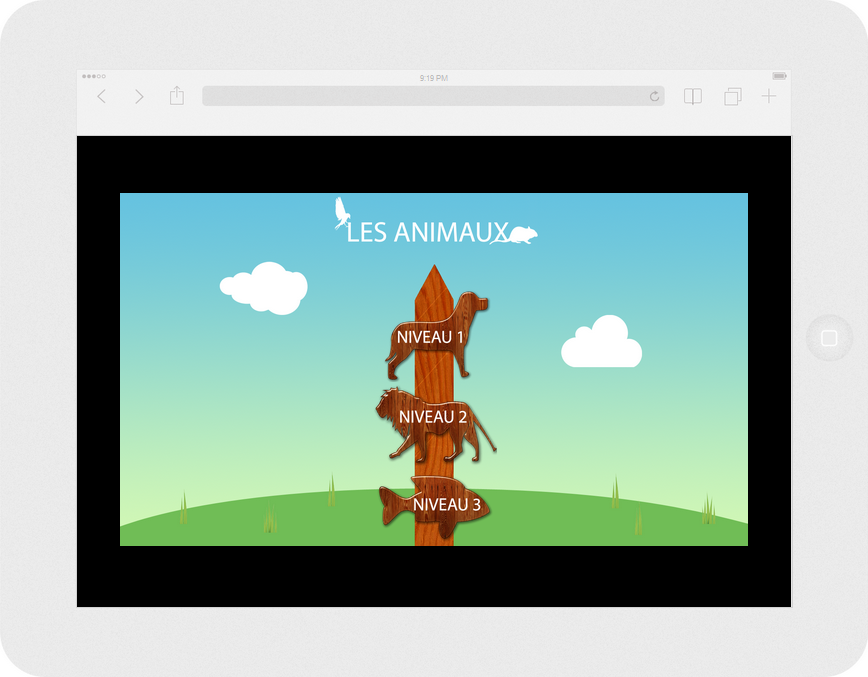
\includegraphics[width=0.8\textwidth]{tablette}\\
\vspace{3cm}
\textbf{Pr\'eambule}
\end{center}

\hspace*{0.6cm}Les jeux sont un bon moyen d'am\'eliorer les comp\'etence logico-math\'ematique et corporelle kinesth\'esique d'une personne. Mais ces effets sont d\'ecupl\'es sur des enfants. Pouss\'e par leur curiosit\'e et leur d\'esirs d'accomplissements, ils feront souvent tout ce qui est en leur pouvoir pour arriver \`a la fin d'un jeu. Ces sentiments, si bien mani\'es, peuvent permettre d'enseigner facilement \'enormement de choses aux enfants qu'ils soit handicap\'es ou non.
\vspace{0.5cm}\\
\hspace*{0.6cm}Notre jeu met le joueur devant un problème d'association logique entre plusieurs images. En d\'ebut de partie, cinq images sont donn\'es au joueur et 3 images en jaune sont quand \`a elles pos\'es devant lui. Le joueur doit alors chercher le lien entre les images qu'il a et celle en jaune.

\newpage
\tableofcontents

\newpage
\section{Pr\'erequis}
1. Un logiciel de d\'ecompression
\begin{itemize}
  \item Winrar
  \item Winzip (Install\'e de base avec windows)
\end{itemize}
2. Un navigateur web 
\begin{itemize}
  \item Internet explorer (Version minimum 9)
  \item Google Chrome (Version minimum 44)
  \item Mozilla Firefox (Version minimum 40)
  \item Safari (Version minimum 5.1)
  \item Opera (Version minimum 12)
  \item iOS (Version minimum 6.1)
  \item Android (Version minimum 2.3)
\end{itemize}
\section{Installation}
\subsection{D\'ecompression}
\hspace*{0.6cm}D\'ecompresser l'archive par un simple clique droit puis extraire ici comme le montre l'image ci-dessous :\\
(Une installation de winrar sera peut-\^etre n\'ecessaire)
\vspace{0.5cm}\\
\fbox{
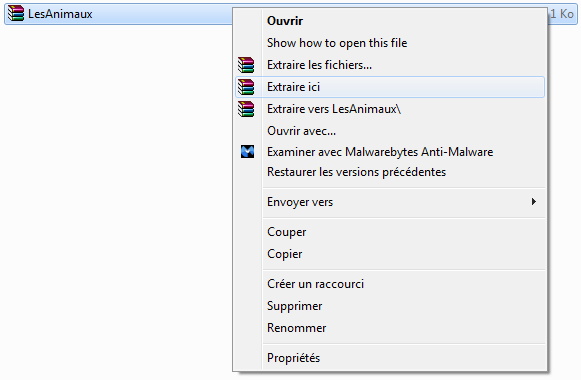
\includegraphics[width=1.0\textwidth]{winrar}\\
}
\subsection{Lancement}
Cliquer ensuite sur le dossier apparu et cliquer sur le fichier nomm\'e "index" ou "index.html" :
\vspace{0.5cm}\\
\fbox{

\includegraphics[width=1.0\textwidth]{index}\\
}
\subsection{Plein \'Ecran}
Il est possible de mettre le jeu en plein \'ecran en cliquant sur F11 une fois le jeu arriv\'e sur l'\'ecran d'accueil. 

\section{Gameplay}



\end{document}